\chapter{Testing Contur}
\label{chapterlabel4}
As already highlighted in the introduction, an important concern when changing live code for optimisation purposes is that we don't unintentionally break or change the final output from \textbf{Contur}.  We identified a robust testing infrastructure as a means to reduce the risk of this happening. In this chapter we slightly digress from profiling and optimisation to discuss the additions we made to \textbf{Contur's} testing infrastructure as part of this project.

\section{Contur Existing Tests}
Prior to work carried out in this thesis, \textbf{Contur} had a limited set of tests\footnote{See initial tests \href{https://gitlab.com/hepcedar/contur/-/tree/49a67e039cf93c88b39dade3dfb7c5f03e780fb2/tests}{here}} implemented within python's pytest framework\cite{pytest}. In the \textbf{Contur} repository these tests can be found in the tests folder. Within the tests folder there are two separate scripts to run tests, \texttt{test\_batch\_submit.py} and \texttt{test\_executables.py}. These test scripts effectively check that the functionality within \textbf{Contur} runs without error, however the tests don't have any visibility on the output of a run (except if the run throws an error before completion).

The main one of these scripts of relevance for the additional tests we will add in subsequent sections is \texttt{test\_executables.py} which checks that \textbf{Contur} runs on a single \textbf{YODA} file and on a grid without errors. To carry out these tests pytest does a single \textbf{YODA} and grid run\footnote{The tests folder contains a single yoda file and a $4 \times 4$ grid for the grid run}. These runs are of relevance to us because we can use their outputs to create regression tests as we will outline in the next section.

\section{Regression Testing}
The simplest test we can put in place to try and mitigate the risks from changes to code is to try and ensure that the change does not alter the final output of a \textbf{Contur} run. This can be achieved by introducing regression testing into \textbf{Contur's} suite of tests. Regression tests will consist of comparing the output of the run we make with the updated code (labelled the target) against the output of a run made before the update to the code (labelled the base). The regression test is passed if our target output is equal to base output\footnote{The target output in this case can be said to regress to base, hence the name regression testing.}. 

Implementing these regression tests within the pytest framework will allow us to carry out the comparison of new results against old results automatically just by running pytest. Thus the regression tests we implemented as part of this project will be of use to other \textbf{Contur} developers to help ensure their changes don't unintentional alter output. Before outlining in greater detail how went about implementing the regression tests it is useful to first give greater clarity on the file format of the results output by \textbf{Contur}.

\subsection{Contur Run Output Format}
Single \textbf{YODA} and grid runs output their results in different file formats. A single \textbf{YODA} run outputs a text file with the results printed in a text file. A example of such an output is shown in figure \ref{fig:contur_txt_output} below. For regression testing purposes we can simple compare that base and target text files are the same excluding the first three lines of the text file which give the location where \textbf{Contur} is running to produce the text file\footnote{This can be seen \ref{fig:contur_txt_output}, if we included these first three lines in our comparison then the single \textbf{YODA} file regression test would always fail whenever \textbf{Contur} is run from a different location which is not something we want to happen.}

\begin{figure}[H]
\centering
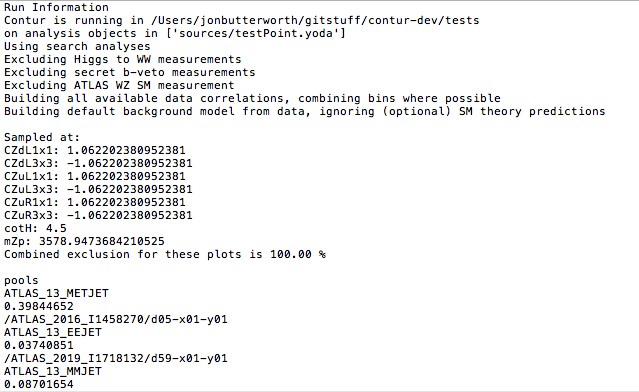
\includegraphics[scale=0.6]{plots/single_yoda_run.png}
\caption{Example output from single yoda run - txt file}
\label{fig:contur_txt_output}
\end{figure}

The grid run returns a pickled\footnote{For further information about pickling objects in Python see \href{https://docs.python.org/3/library/pickle.html}{here}} \say{.map} file. The \say{.map} file contains the \textbf{Contur} \texttt{Depot} object from the run. The \texttt{Depot} object contains all information about a run in its attributes, using the it's \texttt{make\_df} attribute we can create a \textbf{Pandas}\footnote{\textbf{Pandas} is an open source data analysis Python package, further information can be found \href{https://pandas.pydata.org}{here} } \classname{DataFrame} like what we see in figure \ref{fig:contur_df_output} below. For the regression test for the grid we can compare a base and target \classname{DataFrame}.

\begin{figure}[H]
\centering
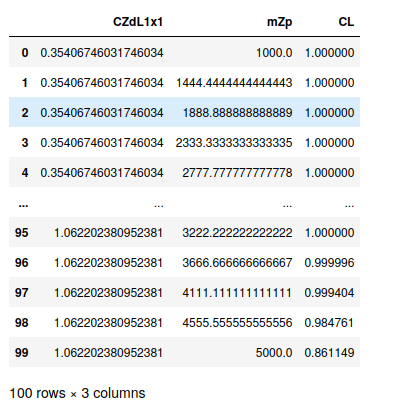
\includegraphics[scale=0.6]{plots/example_data_frame.png}
\caption{Example output from grid run - dataframe}
\label{fig:contur_df_output}
\end{figure}


\subsection{Implementing Regression Tests}
Adding the regression tests\footnote{See commit \href{https://gitlab.com/hepcedar/contur/-/commit/a56006379872ee45c6b7689ce3aeea8ab8fd7435}{a5600637} for the first tests added} to \textbf{Contur's} testing infrastructure is straight forward enough. For the single \textbf{YODA} regression we added the function given in listing \ref{code:single_yoda_regression} to the \texttt{test\_executables.py} script. This function first reads in the base text file and then reads in the target text file created from the run. Then after removing the first three lines from each text file the function checks that the text files are the same.

\begin{code}
\captionof{listing}{Single \texttt{YODA} Regression Test}
\label{code:single_yoda_regression}
\begin{minted}{python}
def test_regression_single_yoda_run():
   args_path = os.path.join(test_dir, 'base.txt')
   with open(args_path) as sf:
       base = sf.read().splitlines(True)
    
   args_path = os.path.join(test_dir, 'target.txt')
   with open(args_path) as sf:
       target = sf.read().splitlines(True)
   assert base[3:] == target[3:]
\end{minted}
\end{code}

The regression test for the grid run is similar to the single \textbf{Contur} regression. We can see the function for the grid regression in listing \ref{code:grid_regression}. Instead of text files this function pickles two map files and then calls the \texttt{Depot.\_build\_frame()} attribute to create a base and target \classname{DataFrame}. We then use \textbf{Pandas's} \texttt{assert\_frame\_equal()}\footnote{See \href{https://pandas.pydata.org/docs/reference/api/pandas.testing.assert_frame_equal.html}{here} for \textbf{Pandas} documentation for this function} function to check if the two \classname{DataFrame} are equal. Using the \texttt{assert\_frame\_equal()} default settings, this test will pass if the numerical differences between any two corresponding cells in the two \classname{DataFrame} is less than $10^{-8}$.

\begin{code}
\captionof{listing}{Grid Regression}
\label{code:grid_regression}
\begin{minted}{python}
def test_regression_grid_run():
    args_path = os.path.join(test_dir, 'base.map')
    with open(args_path, 'rb') as file:
        base = pkl.load(file)._build_frame()
    args_path = os.path.join(test_dir, 'target.map')
    with open(args_path, 'rb') as file:
        target = pkl.load(file)._build_frame()
    assert_frame_equal(base, target)
\end{minted}
\end{code}

\subsection{Including Theory Runs}
In addition to including regression test for the default \textbf{Contur} runs we also added regression tests for the theory runs too. Recall when the theory option is specified \textbf{Contur} includes SM expectations so the theory option will potentially give different output than the default run. The theory regression tests were added using similar functions to listing \ref{code:single_yoda_regression} and \ref{code:grid_regression}.


